\def \imgh {1.5cm}
\def \imgw {1.9cm}

\begin{figure*}
\begin{center}
%%
%%
%%
%%
%%
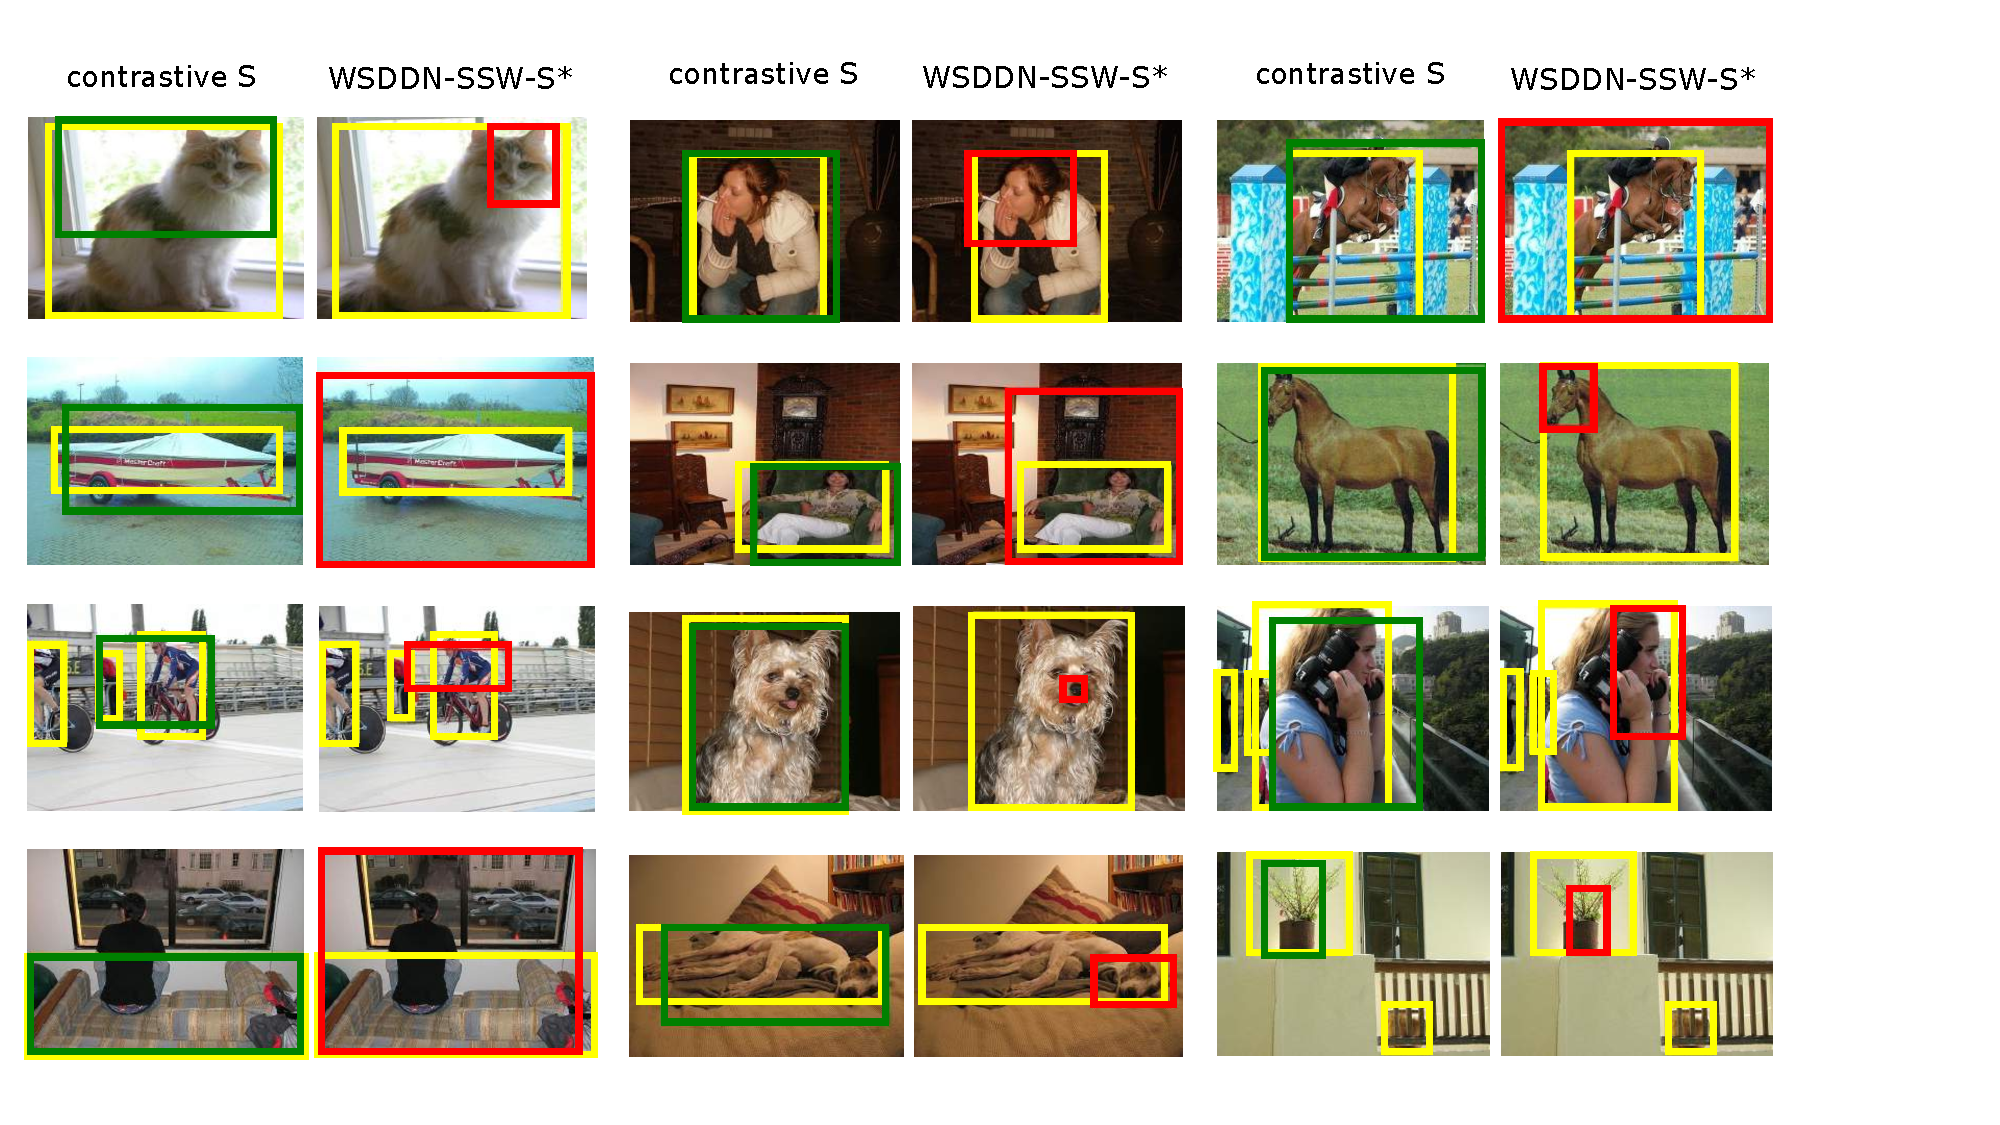
\includegraphics[trim = 0cm 0.8cm 2.8cm 0cm, clip, width=0.98\linewidth] {images/detectionresults_goodbad_1_compressed.pdf}
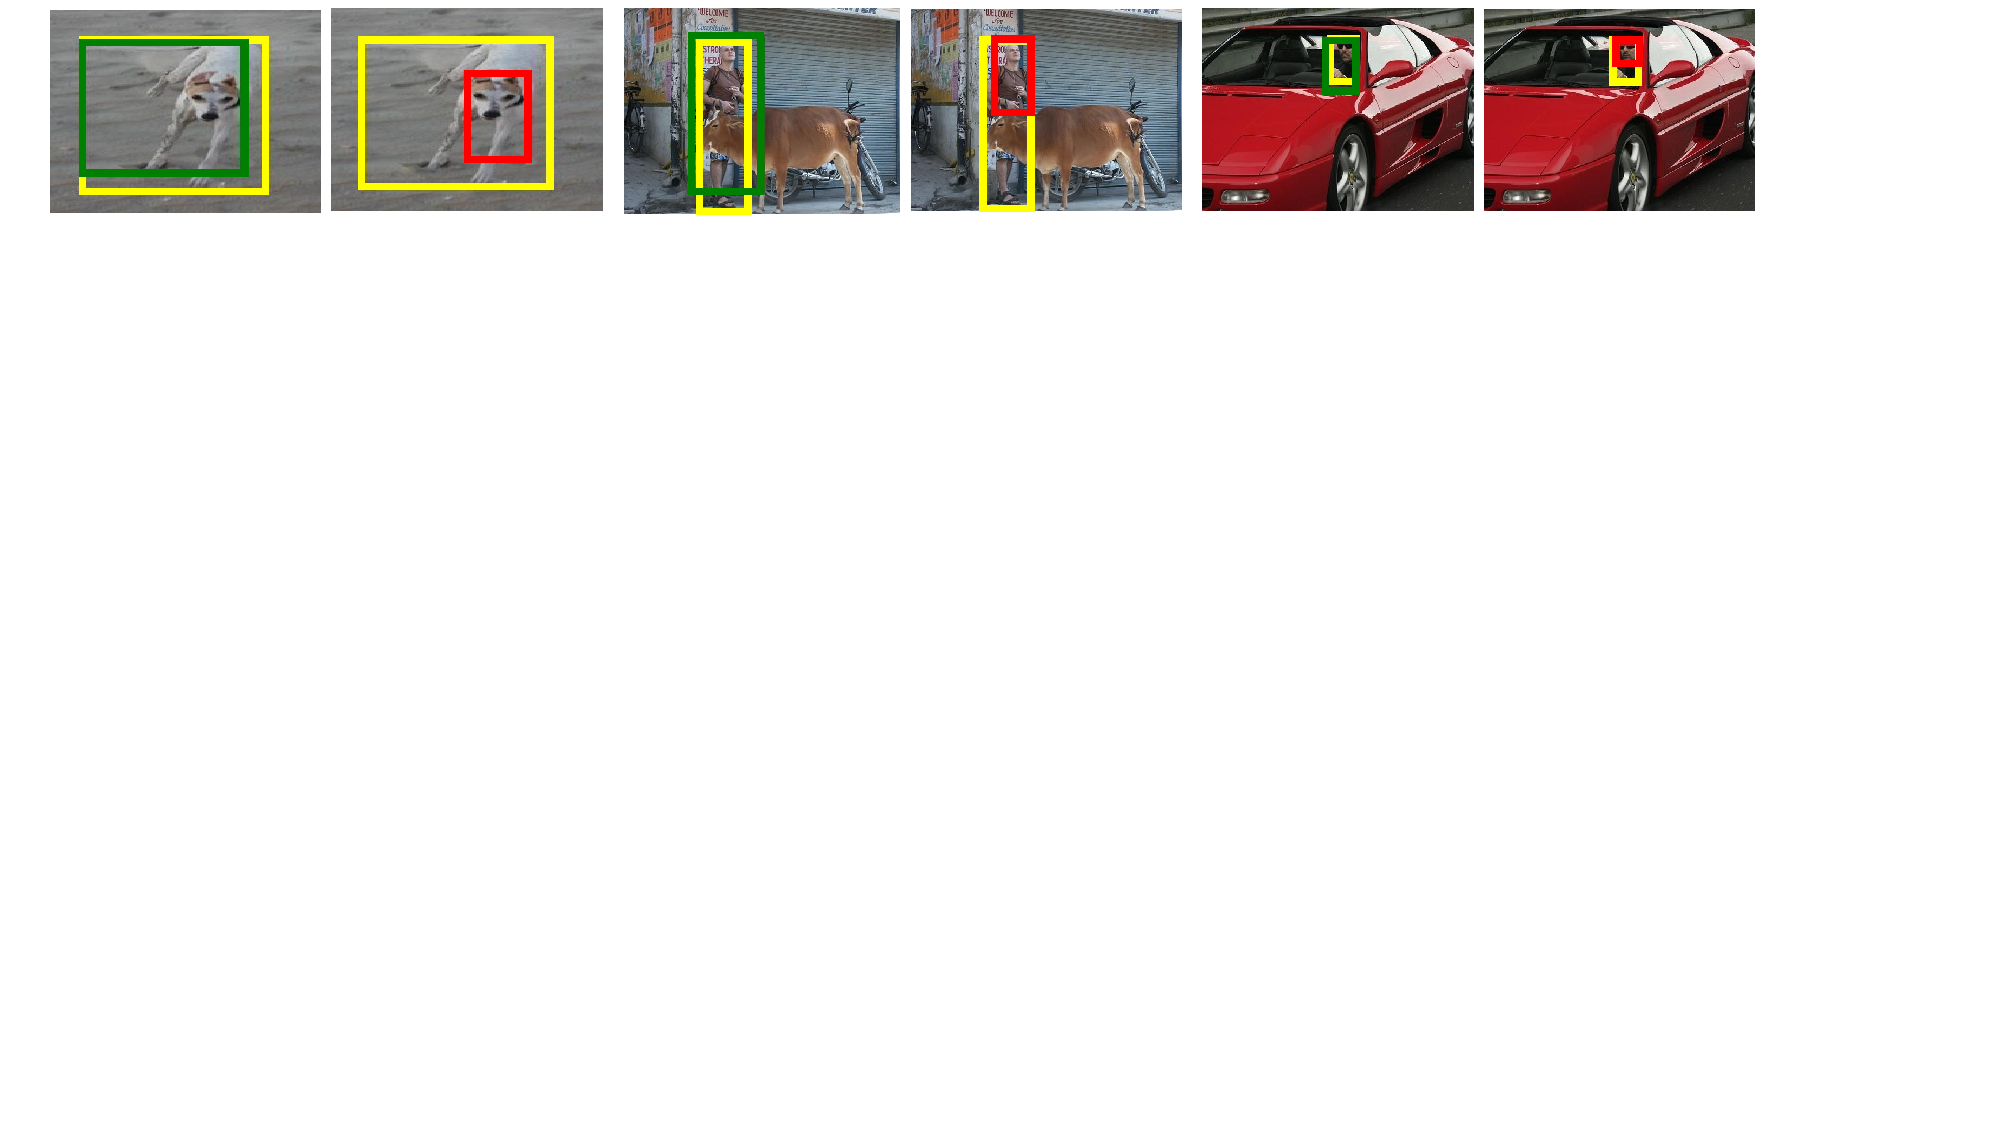
\includegraphics[trim = 0cm 13.5cm 2.8cm 0cm, clip, width=1.0\linewidth] {images/detectionresults_goodbad_4.pdf}
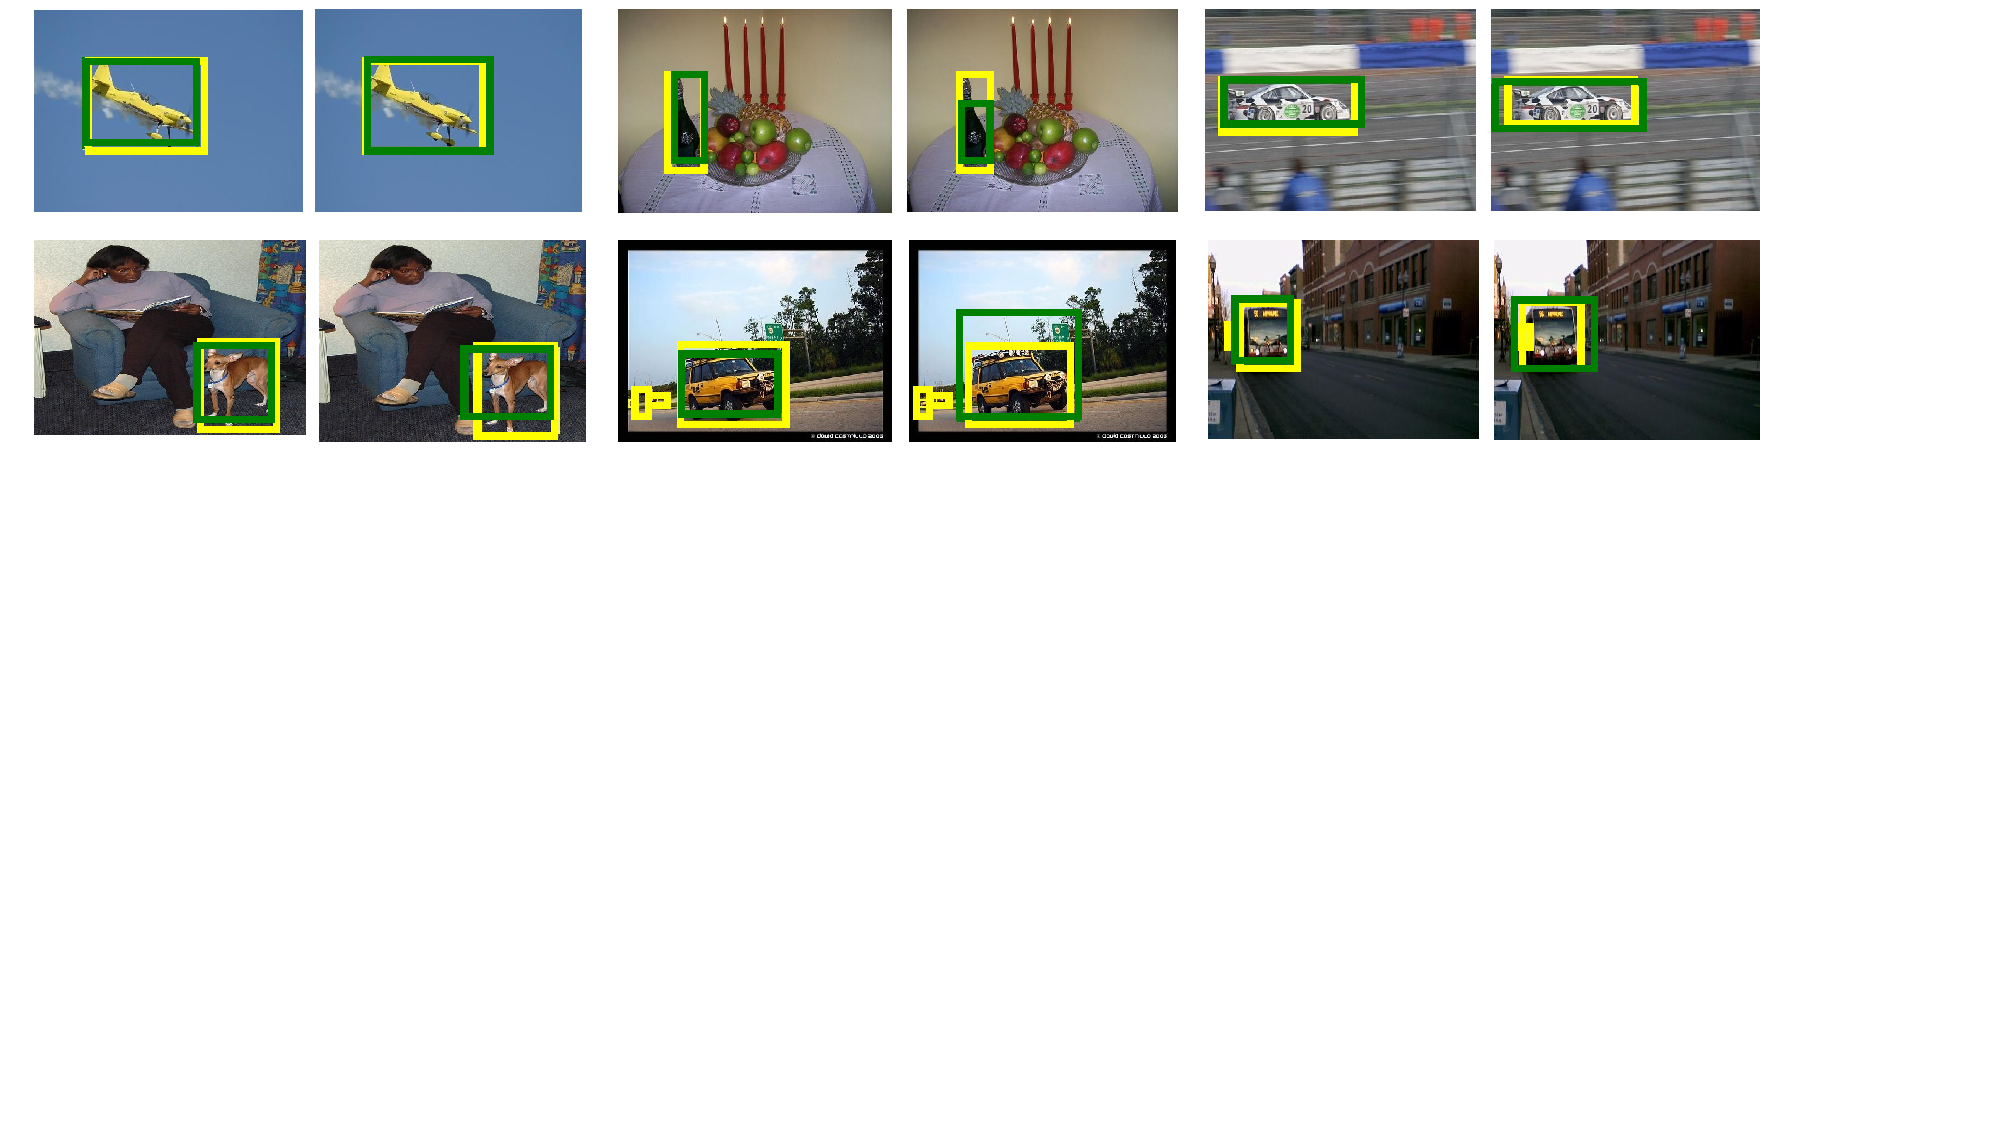
\includegraphics[trim = 0cm 10cm 3cm 0cm, clip, width=0.985\linewidth] {images/detectionresults_goodbad_3.pdf}
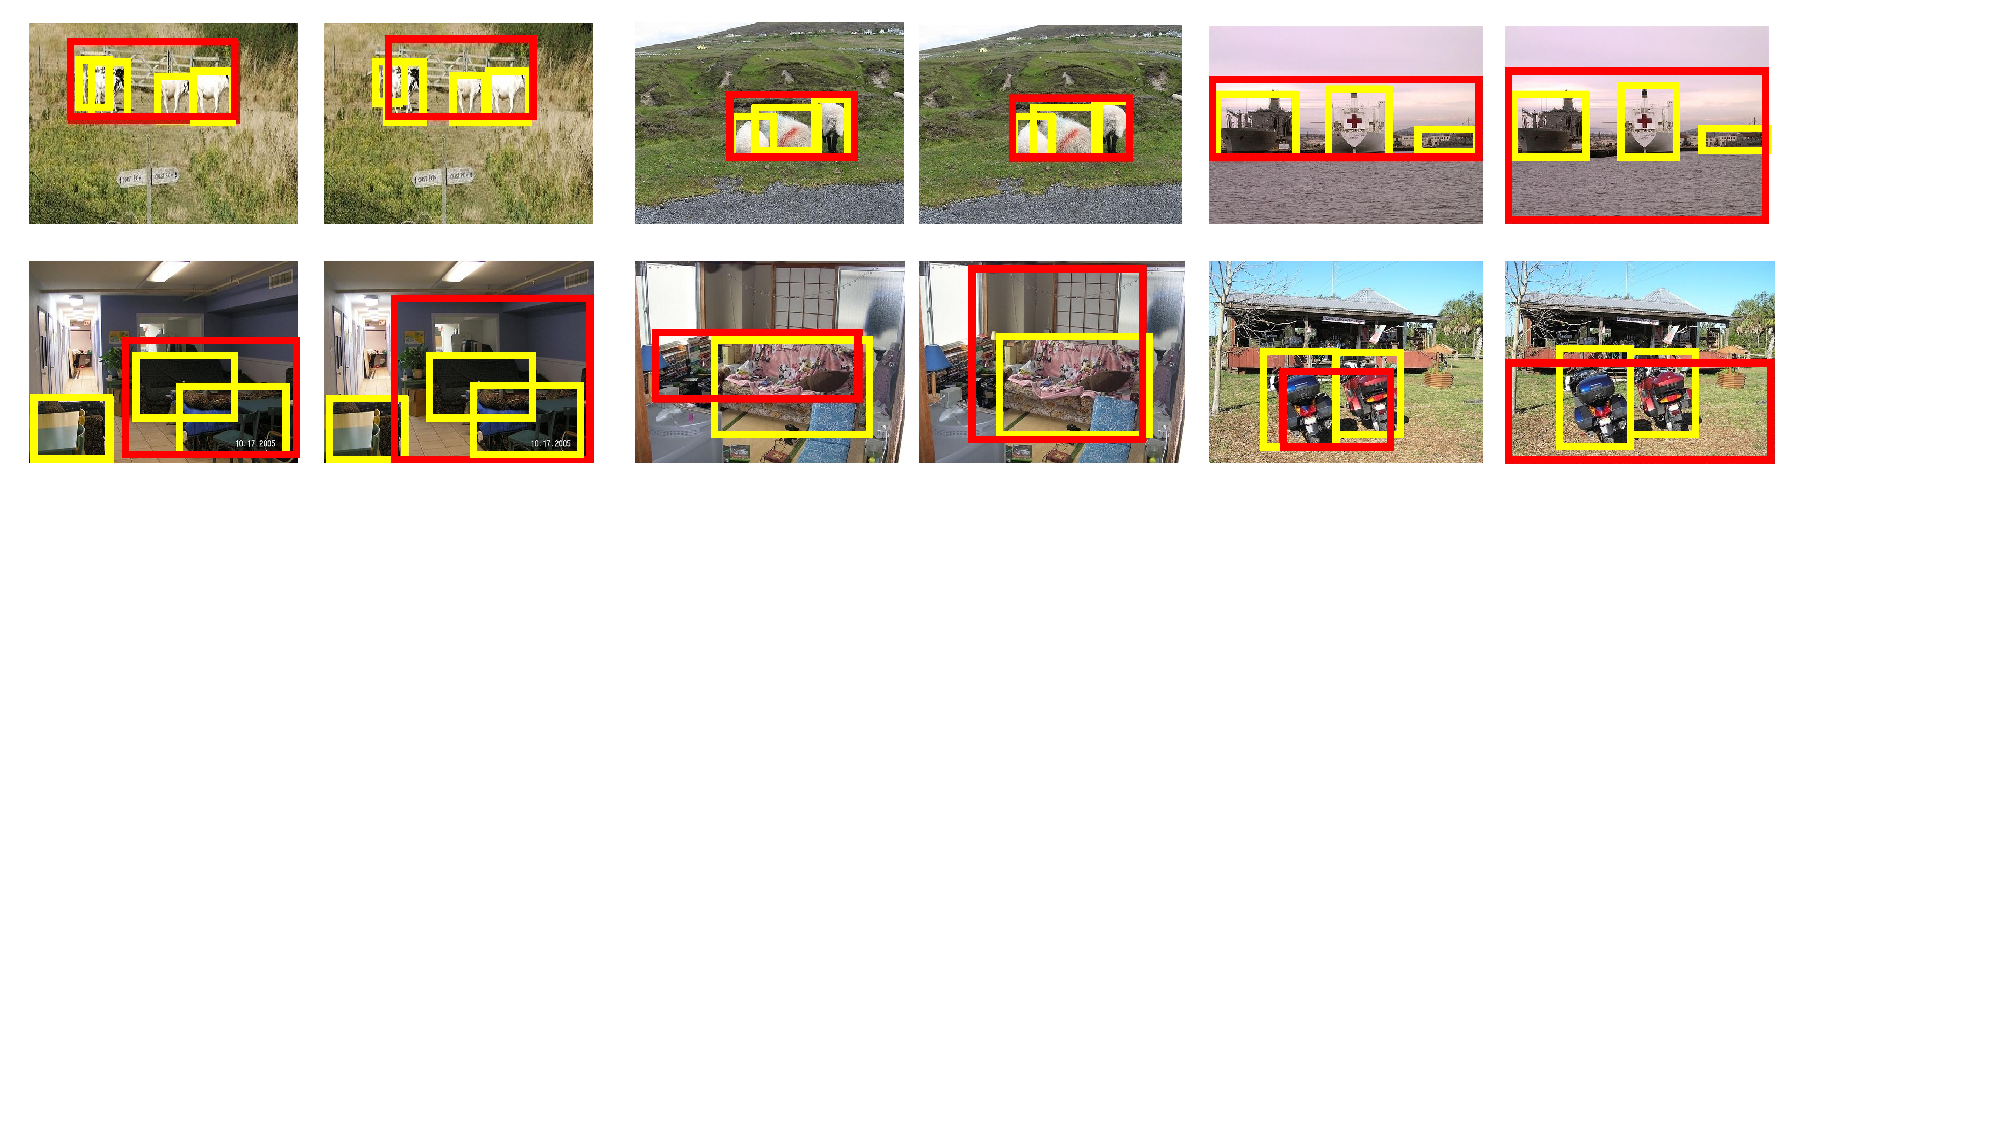
\includegraphics[trim = 0cm 11cm 3cm 0cm, clip, width=0.98\linewidth] {images/detectionresults_goodbad_2.pdf}
\mbox{}\vspace{-.3cm}\\
\end{center}
\caption{The first five rows show localization examples where our method (contrastive S) outperforms WSDDN-SSW-S$^*$ baseline. Two next rows show examples where both methods succeed. The last two rows illustrate failure cases for both methods. Our method often suceeds in localizing correct object boundaries on examples where WSDNN-SSW-S$^*$ is locked to descriminative object parts such as heads of people and animals. Typical failure cases for both methods include images with multiple objects of the same class.}
\label{fig:detexamples}
\end{figure*}

